% Optional new figure, not automatically injected into main.tex/submission.tex.
% Design inspiration: Cao et al., T2AV-Compass, arXiv:2512.21094v3, Figure 1.
\begin{figure*}[t]
  \centering
  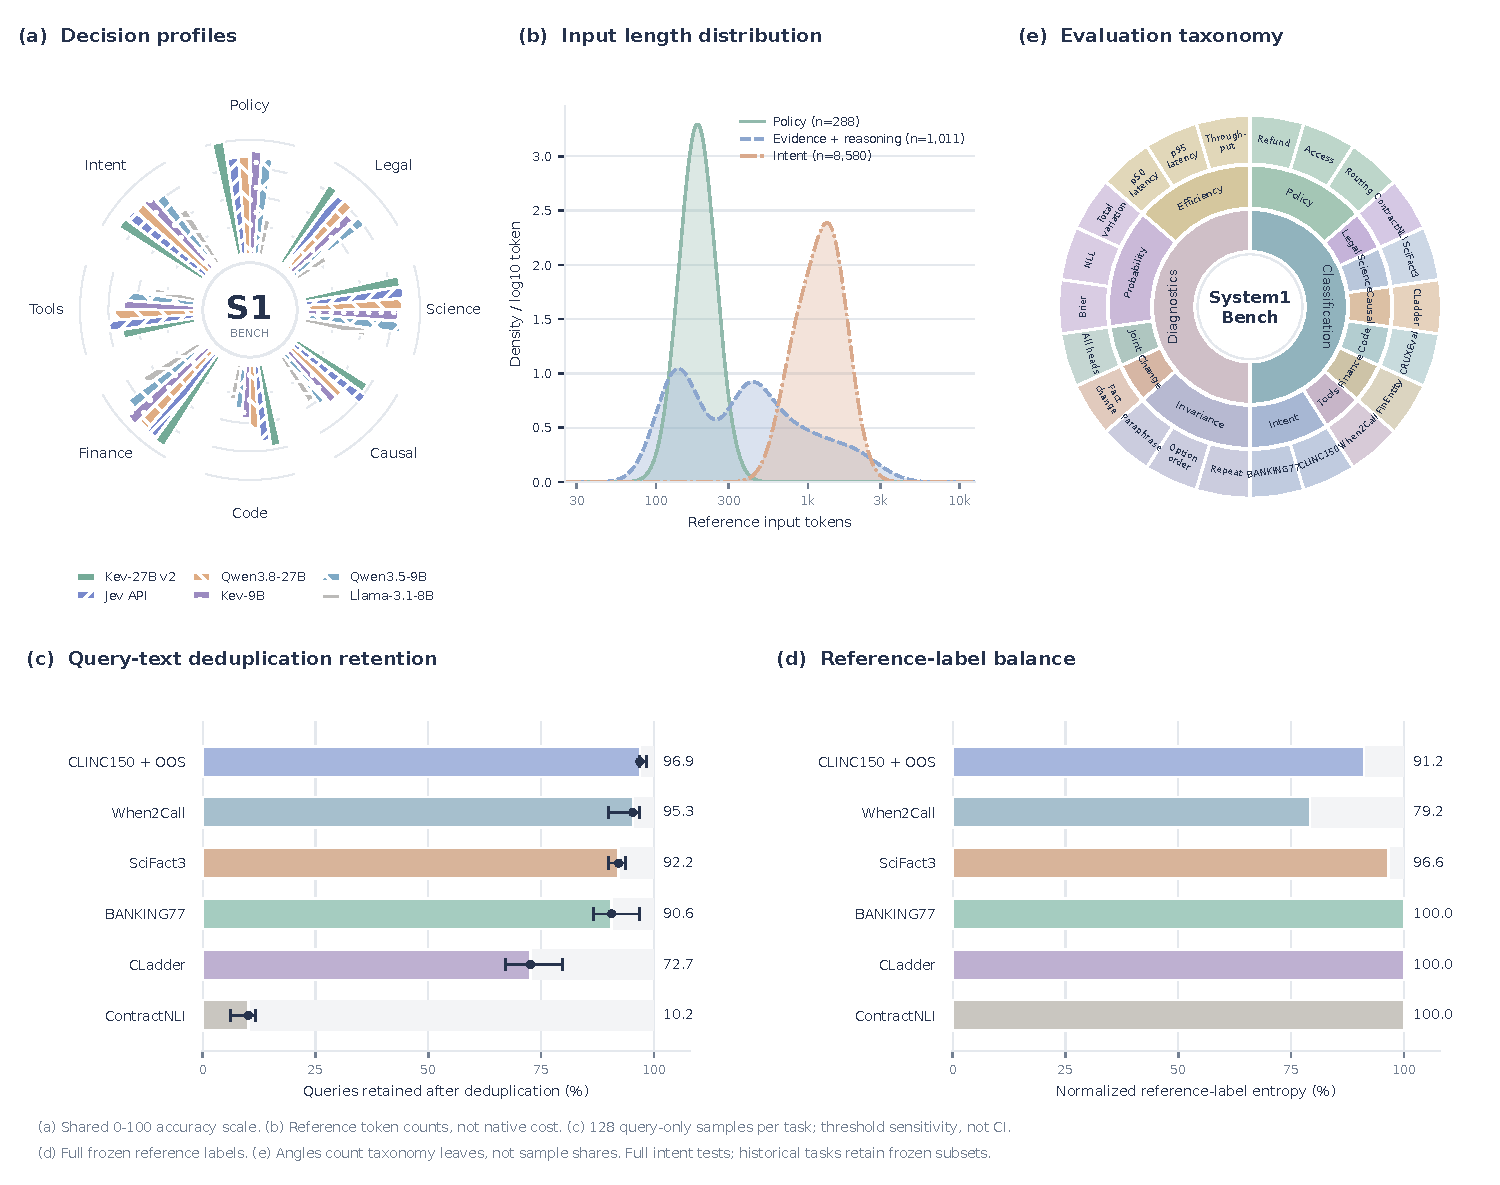
\includegraphics[width=\textwidth]{figures/compass_v1/overview_five_panels.pdf}
  \caption{\textbf{System1Bench: decision profiles, corpus statistics, and evaluation taxonomy.}
  (a) Six representative systems on eight domains, with a shared 0--100 accuracy scale; the full 17-model complete cohort is provided in the accompanying data.
  (b) Gold-free reference request length for 9,879 original classification cases using a common Qwen3.8 tokenizer, including all candidates; these are not native model token costs.
  (c) Query-only semantic retention for 128 deterministically selected queries per task using a pinned MiniLM encoder and cosine threshold 0.80. Lines show sensitivity to thresholds 0.75--0.85, not confidence intervals. ContractNLI reuses hypotheses across distinct contracts; query retention is not whole-corpus diversity.
  (d) Reference-label entropy normalized by the declared ontology, $H(Y)/\log K$, using all scored original cases. Semantic labels, not per-case blinded candidate IDs, are counted; When2Call has three observed classes among four choices.
  (e) Classification tasks and separate diagnostic tracks. Angles count terminal taxonomy leaves, not sample shares or score weights. Diagnostic coverage differs by track.
  Full official intent tests are used; historical tasks retain frozen evaluation subsets. Scores are descriptive point estimates, not evidence of uncontaminated training or statistically significant model differences.}
  \label{fig:compass-overview}
\end{figure*}
